\documentclass[twoside]{book}

% Packages required by doxygen
\usepackage{fixltx2e}
\usepackage{calc}
\usepackage{doxygen}
\usepackage[export]{adjustbox} % also loads graphicx
\usepackage{graphicx}
\usepackage[utf8]{inputenc}
\usepackage{makeidx}
\usepackage{multicol}
\usepackage{multirow}
\PassOptionsToPackage{warn}{textcomp}
\usepackage{textcomp}
\usepackage[nointegrals]{wasysym}
\usepackage[table]{xcolor}

% NLS support packages
\usepackage[spanish]{babel}
% Font selection
\usepackage[T1]{fontenc}
\usepackage[scaled=.90]{helvet}
\usepackage{courier}
\usepackage{amssymb}
\usepackage{sectsty}
\renewcommand{\familydefault}{\sfdefault}
\allsectionsfont{%
  \fontseries{bc}\selectfont%
  \color{darkgray}%
}
\renewcommand{\DoxyLabelFont}{%
  \fontseries{bc}\selectfont%
  \color{darkgray}%
}
\newcommand{\+}{\discretionary{\mbox{\scriptsize$\hookleftarrow$}}{}{}}

% Page & text layout
\usepackage{geometry}
\geometry{%
  a4paper,%
  top=2.5cm,%
  bottom=2.5cm,%
  left=2.5cm,%
  right=2.5cm%
}
\tolerance=750
\hfuzz=15pt
\hbadness=750
\setlength{\emergencystretch}{15pt}
\setlength{\parindent}{0cm}
\setlength{\parskip}{3ex plus 2ex minus 2ex}
\makeatletter
\renewcommand{\paragraph}{%
  \@startsection{paragraph}{4}{0ex}{-1.0ex}{1.0ex}{%
    \normalfont\normalsize\bfseries\SS@parafont%
  }%
}
\renewcommand{\subparagraph}{%
  \@startsection{subparagraph}{5}{0ex}{-1.0ex}{1.0ex}{%
    \normalfont\normalsize\bfseries\SS@subparafont%
  }%
}
\makeatother

% Headers & footers
\usepackage{fancyhdr}
\pagestyle{fancyplain}
\fancyhead[LE]{\fancyplain{}{\bfseries\thepage}}
\fancyhead[CE]{\fancyplain{}{}}
\fancyhead[RE]{\fancyplain{}{\bfseries\leftmark}}
\fancyhead[LO]{\fancyplain{}{\bfseries\rightmark}}
\fancyhead[CO]{\fancyplain{}{}}
\fancyhead[RO]{\fancyplain{}{\bfseries\thepage}}
\fancyfoot[LE]{\fancyplain{}{}}
\fancyfoot[CE]{\fancyplain{}{}}
\fancyfoot[RE]{\fancyplain{}{\bfseries\scriptsize Generado por Doxygen }}
\fancyfoot[LO]{\fancyplain{}{\bfseries\scriptsize Generado por Doxygen }}
\fancyfoot[CO]{\fancyplain{}{}}
\fancyfoot[RO]{\fancyplain{}{}}
\renewcommand{\footrulewidth}{0.4pt}
\renewcommand{\chaptermark}[1]{%
  \markboth{#1}{}%
}
\renewcommand{\sectionmark}[1]{%
  \markright{\thesection\ #1}%
}

% Indices & bibliography
\usepackage{natbib}
\usepackage[titles]{tocloft}
\setcounter{tocdepth}{3}
\setcounter{secnumdepth}{5}
\makeindex

% Hyperlinks (required, but should be loaded last)
\usepackage{ifpdf}
\ifpdf
  \usepackage[pdftex,pagebackref=true]{hyperref}
\else
  \usepackage[ps2pdf,pagebackref=true]{hyperref}
\fi
\hypersetup{%
  colorlinks=true,%
  linkcolor=blue,%
  citecolor=blue,%
  unicode%
}

% Custom commands
\newcommand{\clearemptydoublepage}{%
  \newpage{\pagestyle{empty}\cleardoublepage}%
}

\usepackage{caption}
\captionsetup{labelsep=space,justification=centering,font={bf},singlelinecheck=off,skip=4pt,position=top}

%===== C O N T E N T S =====

\begin{document}

% Titlepage & ToC
\hypersetup{pageanchor=false,
             bookmarksnumbered=true,
             pdfencoding=unicode
            }
\pagenumbering{alph}
\begin{titlepage}
\vspace*{7cm}
\begin{center}%
{\Large Calculadora d’expressions aritmetiques }\\
\vspace*{1cm}
{\large Generado por Doxygen 1.8.12}\\
\end{center}
\end{titlepage}
\clearemptydoublepage
\pagenumbering{roman}
\tableofcontents
\clearemptydoublepage
\pagenumbering{arabic}
\hypersetup{pageanchor=true}

%--- Begin generated contents ---
\chapter{Pràctica Programació 2\+: Calculadora d’expressions aritmètiques}
\label{index}\hypertarget{index}{}En aquesta pràctica hem implementat una calculadora d’expressions aritmètiques que, a més a més, permet definir noves operacions a partir d’operacions ja existents.

Hem fet servir les classes \hyperlink{operacio_8hh}{operacio.\+hh}, \hyperlink{variable_8hh}{variable.\+hh}, \hyperlink{resultat__lectura_8hh}{resultat\+\_\+lectura.\+hh}, \hyperlink{resultat_8hh}{resultat.\+hh}. 
\chapter{Índice de clases}
\section{Lista de clases}
Lista de las clases, estructuras, uniones e interfaces con una breve descripción\+:\begin{DoxyCompactList}
\item\contentsline{section}{\hyperlink{classoperacio}{operacio} \\*Conté les operacions que s’han definit i les opera quan apareixen a una expressió }{\pageref{classoperacio}}{}
\item\contentsline{section}{\hyperlink{classresultat}{resultat} \\*Objecte que representa el resultat d\textquotesingle{}una operació }{\pageref{classresultat}}{}
\item\contentsline{section}{\hyperlink{classresultat__lectura}{resultat\+\_\+lectura} \\*Guarda la informació necessària per entendre i tractar l’entrada de la pràctica }{\pageref{classresultat__lectura}}{}
\item\contentsline{section}{\hyperlink{classvariable}{variable} \\*Conté les variables que s’han definit }{\pageref{classvariable}}{}
\end{DoxyCompactList}

\chapter{Indice de archivos}
\section{Lista de archivos}
Lista de todos los archivos con descripciones breves\+:\begin{DoxyCompactList}
\item\contentsline{section}{\hyperlink{_celula_8cc}{Celula.\+cc} \\*Código de la clase \hyperlink{class_celula}{Celula} }{\pageref{_celula_8cc}}{}
\item\contentsline{section}{\hyperlink{_celula_8hh}{Celula.\+hh} \\*Especificación de la clase \hyperlink{class_celula}{Celula} }{\pageref{_celula_8hh}}{}
\item\contentsline{section}{\hyperlink{_organismo_8cc}{Organismo.\+cc} \\*Código de la clase \hyperlink{class_organismo}{Organismo} }{\pageref{_organismo_8cc}}{}
\item\contentsline{section}{\hyperlink{_organismo_8hh}{Organismo.\+hh} \\*Especificación de la clase \hyperlink{class_organismo}{Organismo} }{\pageref{_organismo_8hh}}{}
\item\contentsline{section}{\hyperlink{pro2_8cc}{pro2.\+cc} \\*Programa principal }{\pageref{pro2_8cc}}{}
\item\contentsline{section}{\hyperlink{readbool_8hh}{readbool.\+hh} \\*Operacion para leer booleanos del canal estandar }{\pageref{readbool_8hh}}{}
\item\contentsline{section}{\hyperlink{_sistema_8cc}{Sistema.\+cc} \\*Código de la clase \hyperlink{class_sistema}{Sistema} }{\pageref{_sistema_8cc}}{}
\item\contentsline{section}{\hyperlink{_sistema_8hh}{Sistema.\+hh} \\*Especificación de la clase \hyperlink{class_sistema}{Sistema} }{\pageref{_sistema_8hh}}{}
\end{DoxyCompactList}

\chapter{Documentación de las clases}
\hypertarget{classoperacio}{}\section{Referencia de la Clase operacio}
\label{classoperacio}\index{operacio@{operacio}}


Conté les operacions que s’han definit i les opera quan apareixen a una expressió  


\subsection*{Métodos públicos}
\begin{DoxyCompactItemize}
\item 
\hyperlink{classoperacio_aa16956dfb69552de3ff43261de600bbe}{operacio} ()
\begin{DoxyCompactList}\small\item\em Constructora per defecte. \end{DoxyCompactList}\item 
bool \hyperlink{classoperacio_aa1f42a80cc416ff33caea9898fe3c9b9}{guardar\+\_\+operacio} (const list$<$ string $>$ \&expressio)
\begin{DoxyCompactList}\small\item\em Serveix per guardar una nova operació \end{DoxyCompactList}\item 
\hyperlink{classresultat}{resultat} \hyperlink{classoperacio_ab64cf3a9e19efd65c2ea3fe276cfabaf}{operar} (list$<$ string $>$ \&op, list$<$ string $>$\+::iterator it)
\begin{DoxyCompactList}\small\item\em Opera una expressio. \end{DoxyCompactList}\end{DoxyCompactItemize}


\subsection{Descripción detallada}
Conté les operacions que s’han definit i les opera quan apareixen a una expressió 

Definición en la línea 12 del archivo operacio.\+hh.



\subsection{Documentación del constructor y destructor}
\hypertarget{classoperacio_aa16956dfb69552de3ff43261de600bbe}{}\label{classoperacio_aa16956dfb69552de3ff43261de600bbe} 
\index{operacio@{operacio}!operacio@{operacio}}
\index{operacio@{operacio}!operacio@{operacio}}
\subsubsection{\texorpdfstring{operacio()}{operacio()}}
{\footnotesize\ttfamily operacio\+::operacio (\begin{DoxyParamCaption}{ }\end{DoxyParamCaption})}



Constructora per defecte. 

\begin{DoxyPrecond}{Precondición}
Cert 
\end{DoxyPrecond}
\begin{DoxyPostcond}{Postcondición}
el p.\+i està buit. 
\end{DoxyPostcond}


\subsection{Documentación de las funciones miembro}
\hypertarget{classoperacio_aa1f42a80cc416ff33caea9898fe3c9b9}{}\label{classoperacio_aa1f42a80cc416ff33caea9898fe3c9b9} 
\index{operacio@{operacio}!guardar\+\_\+operacio@{guardar\+\_\+operacio}}
\index{guardar\+\_\+operacio@{guardar\+\_\+operacio}!operacio@{operacio}}
\subsubsection{\texorpdfstring{guardar\+\_\+operacio()}{guardar\_operacio()}}
{\footnotesize\ttfamily bool operacio\+::guardar\+\_\+operacio (\begin{DoxyParamCaption}\item[{const list$<$ string $>$ \&}]{expressio }\end{DoxyParamCaption})}



Serveix per guardar una nova operació 

\begin{DoxyPrecond}{Precondición}
{\itshape expressio} és una expressió vàlida tal i com s’explicita a l’enunciat de la pràctica. 
\end{DoxyPrecond}
\begin{DoxyPostcond}{Postcondición}
{\itshape true} si ha aconseguit guardar l\textquotesingle{}operacio {\itshape expressio} amb el nom corresponent i treu per pantalla la sortida que indica el enunciat, altrament retorna {\itshape false} 
\end{DoxyPostcond}
\hypertarget{classoperacio_ab64cf3a9e19efd65c2ea3fe276cfabaf}{}\label{classoperacio_ab64cf3a9e19efd65c2ea3fe276cfabaf} 
\index{operacio@{operacio}!operar@{operar}}
\index{operar@{operar}!operacio@{operacio}}
\subsubsection{\texorpdfstring{operar()}{operar()}}
{\footnotesize\ttfamily \hyperlink{classresultat}{resultat} operacio\+::operar (\begin{DoxyParamCaption}\item[{list$<$ string $>$ \&}]{op,  }\item[{list$<$ string $>$\+::iterator}]{it }\end{DoxyParamCaption})}



Opera una expressio. 

\begin{DoxyPrecond}{Precondición}
it = IT, cert 
\end{DoxyPrecond}
\begin{DoxyPostcond}{Postcondición}
Retorna el resultat de l’operació que comença a on apunta IT 
\end{DoxyPostcond}


La documentación para esta clase fue generada a partir del siguiente fichero\+:\begin{DoxyCompactItemize}
\item 
operacio.\+hh\end{DoxyCompactItemize}

\hypertarget{classresultat}{}\section{Referencia de la Clase resultat}
\label{classresultat}\index{resultat@{resultat}}


Objecte que representa el resultat d\textquotesingle{}una operació  


\subsection*{Métodos públicos}
\begin{DoxyCompactItemize}
\item 
\hyperlink{classresultat_a536c47bd86857e3f5bfb26e156cb1877}{resultat} ()
\begin{DoxyCompactList}\small\item\em Constructora per defecte. \end{DoxyCompactList}\item 
bool \hyperlink{classresultat_a3ed548d73663ca956ac2f087c400abe6}{es\+\_\+bool} () const
\begin{DoxyCompactList}\small\item\em Consultora 1. \end{DoxyCompactList}\item 
bool \hyperlink{classresultat_a38e2b83a0bac16445b80e553321d1a61}{es\+\_\+llista} () const
\begin{DoxyCompactList}\small\item\em Consultora 2. \end{DoxyCompactList}\item 
bool \hyperlink{classresultat_a6d111168a77585236466639eb058a1bf}{es\+\_\+enter} () const
\begin{DoxyCompactList}\small\item\em Consultora 3. \end{DoxyCompactList}\item 
bool \hyperlink{classresultat_a82069f4c30872bf0129366d4d998a788}{es\+\_\+indefinit} () const
\begin{DoxyCompactList}\small\item\em Consultora 4. \end{DoxyCompactList}\item 
list$<$ int $>$ \hyperlink{classresultat_ada9590460dcd2d077f48bc3e10ec529e}{c\+\_\+resultat} () const
\begin{DoxyCompactList}\small\item\em Consultora 5. \end{DoxyCompactList}\item 
void \hyperlink{classresultat_adaa9aa55a0a9891a24f7dc04c4c1ebf2}{print} () const
\begin{DoxyCompactList}\small\item\em treu per pantalla la informacio del resultat tal i com explicita l\textquotesingle{}enunciat \end{DoxyCompactList}\end{DoxyCompactItemize}


\subsection{Descripción detallada}
Objecte que representa el resultat d\textquotesingle{}una operació 

Definición en la línea 13 del archivo resultat.\+hh.



\subsection{Documentación del constructor y destructor}
\hypertarget{classresultat_a536c47bd86857e3f5bfb26e156cb1877}{}\label{classresultat_a536c47bd86857e3f5bfb26e156cb1877} 
\index{resultat@{resultat}!resultat@{resultat}}
\index{resultat@{resultat}!resultat@{resultat}}
\subsubsection{\texorpdfstring{resultat()}{resultat()}}
{\footnotesize\ttfamily resultat\+::resultat (\begin{DoxyParamCaption}{ }\end{DoxyParamCaption})}



Constructora per defecte. 

\begin{DoxyPrecond}{Precondición}
Cert 
\end{DoxyPrecond}
\begin{DoxyPostcond}{Postcondición}
el p.\+i és indefinit. 
\end{DoxyPostcond}


\subsection{Documentación de las funciones miembro}
\hypertarget{classresultat_a3ed548d73663ca956ac2f087c400abe6}{}\label{classresultat_a3ed548d73663ca956ac2f087c400abe6} 
\index{resultat@{resultat}!es\+\_\+bool@{es\+\_\+bool}}
\index{es\+\_\+bool@{es\+\_\+bool}!resultat@{resultat}}
\subsubsection{\texorpdfstring{es\+\_\+bool()}{es\_bool()}}
{\footnotesize\ttfamily bool resultat\+::es\+\_\+bool (\begin{DoxyParamCaption}{ }\end{DoxyParamCaption}) const}



Consultora 1. 

\begin{DoxyPrecond}{Precondición}
Cert 
\end{DoxyPrecond}
\begin{DoxyPostcond}{Postcondición}
Retorna {\itshape true} si el p.\+i. representa un bool definit i {\itshape false} si no. 
\end{DoxyPostcond}
\hypertarget{classresultat_a38e2b83a0bac16445b80e553321d1a61}{}\label{classresultat_a38e2b83a0bac16445b80e553321d1a61} 
\index{resultat@{resultat}!es\+\_\+llista@{es\+\_\+llista}}
\index{es\+\_\+llista@{es\+\_\+llista}!resultat@{resultat}}
\subsubsection{\texorpdfstring{es\+\_\+llista()}{es\_llista()}}
{\footnotesize\ttfamily bool resultat\+::es\+\_\+llista (\begin{DoxyParamCaption}{ }\end{DoxyParamCaption}) const}



Consultora 2. 

\begin{DoxyPrecond}{Precondición}
Cert 
\end{DoxyPrecond}
\begin{DoxyPostcond}{Postcondición}
Retorna {\itshape true} si el p.\+i. representa una llista definida i {\itshape false} si no. 
\end{DoxyPostcond}
\hypertarget{classresultat_a6d111168a77585236466639eb058a1bf}{}\label{classresultat_a6d111168a77585236466639eb058a1bf} 
\index{resultat@{resultat}!es\+\_\+enter@{es\+\_\+enter}}
\index{es\+\_\+enter@{es\+\_\+enter}!resultat@{resultat}}
\subsubsection{\texorpdfstring{es\+\_\+enter()}{es\_enter()}}
{\footnotesize\ttfamily bool resultat\+::es\+\_\+enter (\begin{DoxyParamCaption}{ }\end{DoxyParamCaption}) const}



Consultora 3. 

\begin{DoxyPrecond}{Precondición}
Cert 
\end{DoxyPrecond}
\begin{DoxyPostcond}{Postcondición}
Retorna {\itshape true} si el p.\+i. representa un enter definit i {\itshape false} si no. 
\end{DoxyPostcond}
\hypertarget{classresultat_a82069f4c30872bf0129366d4d998a788}{}\label{classresultat_a82069f4c30872bf0129366d4d998a788} 
\index{resultat@{resultat}!es\+\_\+indefinit@{es\+\_\+indefinit}}
\index{es\+\_\+indefinit@{es\+\_\+indefinit}!resultat@{resultat}}
\subsubsection{\texorpdfstring{es\+\_\+indefinit()}{es\_indefinit()}}
{\footnotesize\ttfamily bool resultat\+::es\+\_\+indefinit (\begin{DoxyParamCaption}{ }\end{DoxyParamCaption}) const}



Consultora 4. 

\begin{DoxyPrecond}{Precondición}
Cert 
\end{DoxyPrecond}
\begin{DoxyPostcond}{Postcondición}
Retorna {\itshape true} si el p.\+i. es indefinit i {\itshape false} si no. 
\end{DoxyPostcond}
\hypertarget{classresultat_ada9590460dcd2d077f48bc3e10ec529e}{}\label{classresultat_ada9590460dcd2d077f48bc3e10ec529e} 
\index{resultat@{resultat}!c\+\_\+resultat@{c\+\_\+resultat}}
\index{c\+\_\+resultat@{c\+\_\+resultat}!resultat@{resultat}}
\subsubsection{\texorpdfstring{c\+\_\+resultat()}{c\_resultat()}}
{\footnotesize\ttfamily list$<$int$>$ resultat\+::c\+\_\+resultat (\begin{DoxyParamCaption}{ }\end{DoxyParamCaption}) const}



Consultora 5. 

\begin{DoxyPrecond}{Precondición}
El p.\+i. no és indefinit 
\end{DoxyPrecond}
\begin{DoxyPostcond}{Postcondición}
Retorna el resultat 
\end{DoxyPostcond}
\hypertarget{classresultat_adaa9aa55a0a9891a24f7dc04c4c1ebf2}{}\label{classresultat_adaa9aa55a0a9891a24f7dc04c4c1ebf2} 
\index{resultat@{resultat}!print@{print}}
\index{print@{print}!resultat@{resultat}}
\subsubsection{\texorpdfstring{print()}{print()}}
{\footnotesize\ttfamily void resultat\+::print (\begin{DoxyParamCaption}{ }\end{DoxyParamCaption}) const}



treu per pantalla la informacio del resultat tal i com explicita l\textquotesingle{}enunciat 

\begin{DoxyPrecond}{Precondición}
Cert 
\end{DoxyPrecond}
\begin{DoxyPostcond}{Postcondición}
En el canal estandar de sortida es troba la informacio del resultat tal i com explicita l\textquotesingle{}enunciat 
\end{DoxyPostcond}


La documentación para esta clase fue generada a partir del siguiente fichero\+:\begin{DoxyCompactItemize}
\item 
\hyperlink{resultat_8hh}{resultat.\+hh}\end{DoxyCompactItemize}

\hypertarget{classresultat__lectura}{}\section{Referencia de la Clase resultat\+\_\+lectura}
\label{classresultat__lectura}\index{resultat\+\_\+lectura@{resultat\+\_\+lectura}}


Guarda la informació necessària per entendre i tractar l’entrada de la pràctica.  


\subsection*{Métodos públicos}
\begin{DoxyCompactItemize}
\item 
\hyperlink{classresultat__lectura_a73ef39653019fabadde9454451121b3f}{resultat\+\_\+lectura} ()
\begin{DoxyCompactList}\small\item\em Constructora. L’objecte creat conté l’entrada i informació sobre aquesta. \end{DoxyCompactList}\item 
bool \hyperlink{classresultat__lectura_a4c84ef4ddea623e7a680c639c084d11d}{es\+\_\+def\+\_\+var} () const
\begin{DoxyCompactList}\small\item\em Consultora 1. \end{DoxyCompactList}\item 
bool \hyperlink{classresultat__lectura_ac1f77e1379c99557c3bfdf2d627594f0}{es\+\_\+def\+\_\+op} () const
\begin{DoxyCompactList}\small\item\em Consultora 2. \end{DoxyCompactList}\item 
bool \hyperlink{classresultat__lectura_a0e73a239ad6dd63b591105a5553bef6f}{es\+\_\+expressio} () const
\begin{DoxyCompactList}\small\item\em Consultora 3. \end{DoxyCompactList}\item 
list$<$ string $>$ \hyperlink{classresultat__lectura_a2b6b1c0d200ea75619f7ad50600551c6}{entrada} () const
\begin{DoxyCompactList}\small\item\em Consultora 4. \end{DoxyCompactList}\item 
bool \hyperlink{classresultat__lectura_a178d0aae65fbce754ec5d99a04732bf0}{fi\+\_\+entrada} () const
\begin{DoxyCompactList}\small\item\em Consultora 5. \end{DoxyCompactList}\end{DoxyCompactItemize}


\subsection{Descripción detallada}
Guarda la informació necessària per entendre i tractar l’entrada de la pràctica. 

Definición en la línea 14 del archivo resultat\+\_\+lectura.\+hh.



\subsection{Documentación del constructor y destructor}
\hypertarget{classresultat__lectura_a73ef39653019fabadde9454451121b3f}{}\label{classresultat__lectura_a73ef39653019fabadde9454451121b3f} 
\index{resultat\+\_\+lectura@{resultat\+\_\+lectura}!resultat\+\_\+lectura@{resultat\+\_\+lectura}}
\index{resultat\+\_\+lectura@{resultat\+\_\+lectura}!resultat\+\_\+lectura@{resultat\+\_\+lectura}}
\subsubsection{\texorpdfstring{resultat\+\_\+lectura()}{resultat\_lectura()}}
{\footnotesize\ttfamily resultat\+\_\+lectura\+::resultat\+\_\+lectura (\begin{DoxyParamCaption}{ }\end{DoxyParamCaption})}



Constructora. L’objecte creat conté l’entrada i informació sobre aquesta. 

\begin{DoxyPrecond}{Precondición}
Al canal estàndard d’entrada hi ha una expressió o definició tal i com especifica l’enunciat 
\end{DoxyPrecond}
\begin{DoxyPostcond}{Postcondición}
L’objecte \hyperlink{classresultat__lectura}{resultat\+\_\+lectura} creat conté l’entrada i informació sobre quin tipus d’entrada és\+: una expressió, una definició d’operació o una definició de variable. 
\end{DoxyPostcond}


\subsection{Documentación de las funciones miembro}
\hypertarget{classresultat__lectura_a4c84ef4ddea623e7a680c639c084d11d}{}\label{classresultat__lectura_a4c84ef4ddea623e7a680c639c084d11d} 
\index{resultat\+\_\+lectura@{resultat\+\_\+lectura}!es\+\_\+def\+\_\+var@{es\+\_\+def\+\_\+var}}
\index{es\+\_\+def\+\_\+var@{es\+\_\+def\+\_\+var}!resultat\+\_\+lectura@{resultat\+\_\+lectura}}
\subsubsection{\texorpdfstring{es\+\_\+def\+\_\+var()}{es\_def\_var()}}
{\footnotesize\ttfamily bool resultat\+\_\+lectura\+::es\+\_\+def\+\_\+var (\begin{DoxyParamCaption}{ }\end{DoxyParamCaption}) const}



Consultora 1. 

\begin{DoxyPrecond}{Precondición}
Cert 
\end{DoxyPrecond}
\begin{DoxyPostcond}{Postcondición}
Retorna {\itshape true} si el p.\+i. representa una entrada que defineix una variable i {\itshape false} si no. 
\end{DoxyPostcond}
\hypertarget{classresultat__lectura_ac1f77e1379c99557c3bfdf2d627594f0}{}\label{classresultat__lectura_ac1f77e1379c99557c3bfdf2d627594f0} 
\index{resultat\+\_\+lectura@{resultat\+\_\+lectura}!es\+\_\+def\+\_\+op@{es\+\_\+def\+\_\+op}}
\index{es\+\_\+def\+\_\+op@{es\+\_\+def\+\_\+op}!resultat\+\_\+lectura@{resultat\+\_\+lectura}}
\subsubsection{\texorpdfstring{es\+\_\+def\+\_\+op()}{es\_def\_op()}}
{\footnotesize\ttfamily bool resultat\+\_\+lectura\+::es\+\_\+def\+\_\+op (\begin{DoxyParamCaption}{ }\end{DoxyParamCaption}) const}



Consultora 2. 

\begin{DoxyPrecond}{Precondición}
Cert 
\end{DoxyPrecond}
\begin{DoxyPostcond}{Postcondición}
Retorna {\itshape true} si el p.\+i. representa una entrada que defineix una operació i {\itshape false} si no. 
\end{DoxyPostcond}
\hypertarget{classresultat__lectura_a0e73a239ad6dd63b591105a5553bef6f}{}\label{classresultat__lectura_a0e73a239ad6dd63b591105a5553bef6f} 
\index{resultat\+\_\+lectura@{resultat\+\_\+lectura}!es\+\_\+expressio@{es\+\_\+expressio}}
\index{es\+\_\+expressio@{es\+\_\+expressio}!resultat\+\_\+lectura@{resultat\+\_\+lectura}}
\subsubsection{\texorpdfstring{es\+\_\+expressio()}{es\_expressio()}}
{\footnotesize\ttfamily bool resultat\+\_\+lectura\+::es\+\_\+expressio (\begin{DoxyParamCaption}{ }\end{DoxyParamCaption}) const}



Consultora 3. 

\begin{DoxyPrecond}{Precondición}
Cert 
\end{DoxyPrecond}
\begin{DoxyPostcond}{Postcondición}
Retorna {\itshape true} si el p.\+i. representa una entrada que es una expressio i {\itshape false} si no. 
\end{DoxyPostcond}
\hypertarget{classresultat__lectura_a2b6b1c0d200ea75619f7ad50600551c6}{}\label{classresultat__lectura_a2b6b1c0d200ea75619f7ad50600551c6} 
\index{resultat\+\_\+lectura@{resultat\+\_\+lectura}!entrada@{entrada}}
\index{entrada@{entrada}!resultat\+\_\+lectura@{resultat\+\_\+lectura}}
\subsubsection{\texorpdfstring{entrada()}{entrada()}}
{\footnotesize\ttfamily list$<$string$>$ resultat\+\_\+lectura\+::entrada (\begin{DoxyParamCaption}{ }\end{DoxyParamCaption}) const}



Consultora 4. 

\begin{DoxyPrecond}{Precondición}
el p.\+i no esta buit 
\end{DoxyPrecond}
\begin{DoxyPostcond}{Postcondición}
Retorna l’entrada en el format més adient segons el tipus. 
\end{DoxyPostcond}
\hypertarget{classresultat__lectura_a178d0aae65fbce754ec5d99a04732bf0}{}\label{classresultat__lectura_a178d0aae65fbce754ec5d99a04732bf0} 
\index{resultat\+\_\+lectura@{resultat\+\_\+lectura}!fi\+\_\+entrada@{fi\+\_\+entrada}}
\index{fi\+\_\+entrada@{fi\+\_\+entrada}!resultat\+\_\+lectura@{resultat\+\_\+lectura}}
\subsubsection{\texorpdfstring{fi\+\_\+entrada()}{fi\_entrada()}}
{\footnotesize\ttfamily bool resultat\+\_\+lectura\+::fi\+\_\+entrada (\begin{DoxyParamCaption}{ }\end{DoxyParamCaption}) const}



Consultora 5. 

\begin{DoxyPrecond}{Precondición}
el p.\+i no esta buit 
\end{DoxyPrecond}
\begin{DoxyPostcond}{Postcondición}
Retorna {\itshape true} si el p.\+i. representa una entrada que senyalitza el final de l\textquotesingle{}entrada i {\itshape false} si no. 
\end{DoxyPostcond}


La documentación para esta clase fue generada a partir del siguiente fichero\+:\begin{DoxyCompactItemize}
\item 
\hyperlink{resultat__lectura_8hh}{resultat\+\_\+lectura.\+hh}\end{DoxyCompactItemize}

\hypertarget{classvariable}{}\section{Referencia de la Clase variable}
\label{classvariable}\index{variable@{variable}}


Conté les variables que s’han definit.  


\subsection*{Métodos públicos}
\begin{DoxyCompactItemize}
\item 
\hyperlink{classvariable_a424009148a020b406a8a5ecefa854edc}{variable} ()
\begin{DoxyCompactList}\small\item\em Constructora per defecte. \end{DoxyCompactList}\item 
bool \hyperlink{classvariable_ac8e2c3022d51e243b4c336c023300d28}{guardar\+\_\+variable} (string nom, const \hyperlink{classresultat}{resultat} \&r)
\begin{DoxyCompactList}\small\item\em Serveix per guardar una nova variable. \end{DoxyCompactList}\item 
bool \hyperlink{classvariable_a0b8c6b4971c4f88aa6554e72a76b23fc}{consultar\+\_\+var} (const list$<$ string $>$ \&op, list$<$ string $>$\+::iterator it) const
\begin{DoxyCompactList}\small\item\em Serveix per consultar si existeix una variable amb el nom {\itshape nom} \end{DoxyCompactList}\item 
\hyperlink{classresultat}{resultat} \hyperlink{classvariable_a1d4aa21d6874589f26ec2e7bf08d3e67}{buscar} (const list$<$ string $>$ \&op, list$<$ string $>$\+::iterator it) const
\begin{DoxyCompactList}\small\item\em Retorna el resultat que representa una variable. \end{DoxyCompactList}\end{DoxyCompactItemize}


\subsection{Descripción detallada}
Conté les variables que s’han definit. 

Definición en la línea 13 del archivo variable.\+hh.



\subsection{Documentación del constructor y destructor}
\hypertarget{classvariable_a424009148a020b406a8a5ecefa854edc}{}\label{classvariable_a424009148a020b406a8a5ecefa854edc} 
\index{variable@{variable}!variable@{variable}}
\index{variable@{variable}!variable@{variable}}
\subsubsection{\texorpdfstring{variable()}{variable()}}
{\footnotesize\ttfamily variable\+::variable (\begin{DoxyParamCaption}{ }\end{DoxyParamCaption})}



Constructora per defecte. 

\begin{DoxyPrecond}{Precondición}
Cert 
\end{DoxyPrecond}
\begin{DoxyPostcond}{Postcondición}
el p.\+i està buit. 
\end{DoxyPostcond}


\subsection{Documentación de las funciones miembro}
\hypertarget{classvariable_ac8e2c3022d51e243b4c336c023300d28}{}\label{classvariable_ac8e2c3022d51e243b4c336c023300d28} 
\index{variable@{variable}!guardar\+\_\+variable@{guardar\+\_\+variable}}
\index{guardar\+\_\+variable@{guardar\+\_\+variable}!variable@{variable}}
\subsubsection{\texorpdfstring{guardar\+\_\+variable()}{guardar\_variable()}}
{\footnotesize\ttfamily bool variable\+::guardar\+\_\+variable (\begin{DoxyParamCaption}\item[{string}]{nom,  }\item[{const \hyperlink{classresultat}{resultat} \&}]{r }\end{DoxyParamCaption})}



Serveix per guardar una nova variable. 

\begin{DoxyPrecond}{Precondición}
Cert 
\end{DoxyPrecond}
\begin{DoxyPostcond}{Postcondición}
retorna {\itshape true} si ha aconseguit guardar el resultat {\itshape R} amb el nom {\itshape nom} i treu per pantalla la sortida que indica el enunciat, altrament retorna {\itshape false} 
\end{DoxyPostcond}
\hypertarget{classvariable_a0b8c6b4971c4f88aa6554e72a76b23fc}{}\label{classvariable_a0b8c6b4971c4f88aa6554e72a76b23fc} 
\index{variable@{variable}!consultar\+\_\+var@{consultar\+\_\+var}}
\index{consultar\+\_\+var@{consultar\+\_\+var}!variable@{variable}}
\subsubsection{\texorpdfstring{consultar\+\_\+var()}{consultar\_var()}}
{\footnotesize\ttfamily bool variable\+::consultar\+\_\+var (\begin{DoxyParamCaption}\item[{const list$<$ string $>$ \&}]{op,  }\item[{list$<$ string $>$\+::iterator}]{it }\end{DoxyParamCaption}) const}



Serveix per consultar si existeix una variable amb el nom {\itshape nom} 

\begin{DoxyPrecond}{Precondición}
cert 
\end{DoxyPrecond}
\begin{DoxyPostcond}{Postcondición}
retorna {\itshape true} si existeix una variable amb el nom {\itshape nom}, altrament retorna {\itshape false} 
\end{DoxyPostcond}
\hypertarget{classvariable_a1d4aa21d6874589f26ec2e7bf08d3e67}{}\label{classvariable_a1d4aa21d6874589f26ec2e7bf08d3e67} 
\index{variable@{variable}!buscar@{buscar}}
\index{buscar@{buscar}!variable@{variable}}
\subsubsection{\texorpdfstring{buscar()}{buscar()}}
{\footnotesize\ttfamily \hyperlink{classresultat}{resultat} variable\+::buscar (\begin{DoxyParamCaption}\item[{const list$<$ string $>$ \&}]{op,  }\item[{list$<$ string $>$\+::iterator}]{it }\end{DoxyParamCaption}) const}



Retorna el resultat que representa una variable. 

\begin{DoxyPrecond}{Precondición}
Cert, 
\end{DoxyPrecond}
\begin{DoxyPostcond}{Postcondición}
Retorna el resultat que representa la variable apuntada per {\itshape it} 
\end{DoxyPostcond}


La documentación para esta clase fue generada a partir del siguiente fichero\+:\begin{DoxyCompactItemize}
\item 
variable.\+hh\end{DoxyCompactItemize}

\chapter{Documentación de archivos}
\hypertarget{main_8cc}{}\section{Referencia del Archivo main.\+cc}
\label{main_8cc}\index{main.\+cc@{main.\+cc}}


Programa principal para la practica {\itshape Calculadora d’expressions aritmetiques}.  


Dependencia gráfica adjunta para main.\+cc\+:\nopagebreak
\begin{figure}[H]
\begin{center}
\leavevmode
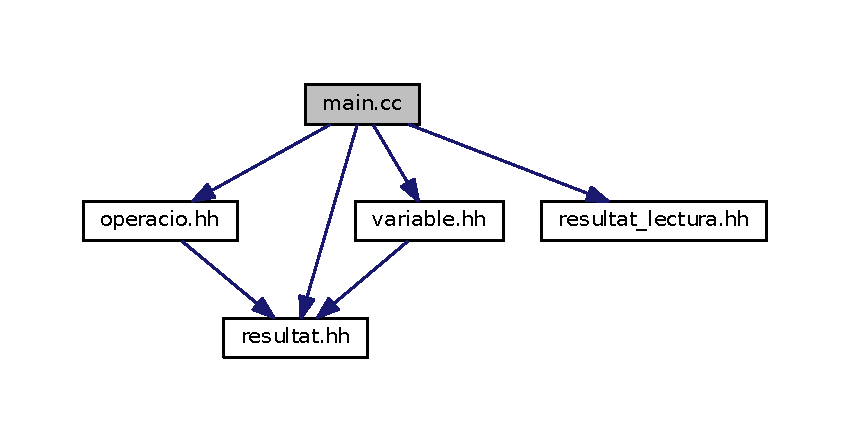
\includegraphics[width=350pt]{main_8cc__incl}
\end{center}
\end{figure}
\subsection*{Funciones}
\begin{DoxyCompactItemize}
\item 
\hyperlink{classresultat}{resultat} \hyperlink{main_8cc_a8618a4d38a75efdcc6be493e3b42907f}{avaluar} (list$<$ string $>$ \&op, list$<$ string $>$\+::iterator \&it)
\begin{DoxyCompactList}\small\item\em Avalua una expressió \end{DoxyCompactList}\item 
int \hyperlink{main_8cc_ae66f6b31b5ad750f1fe042a706a4e3d4}{main} ()
\begin{DoxyCompactList}\small\item\em Programa principial de la pràctica. \end{DoxyCompactList}\end{DoxyCompactItemize}


\subsection{Descripción detallada}
Programa principal para la practica {\itshape Calculadora d’expressions aritmetiques}. 



\subsection{Documentación de las funciones}
\hypertarget{main_8cc_a8618a4d38a75efdcc6be493e3b42907f}{}\label{main_8cc_a8618a4d38a75efdcc6be493e3b42907f} 
\index{main.\+cc@{main.\+cc}!avaluar@{avaluar}}
\index{avaluar@{avaluar}!main.\+cc@{main.\+cc}}
\subsubsection{\texorpdfstring{avaluar()}{avaluar()}}
{\footnotesize\ttfamily \hyperlink{classresultat}{resultat} avaluar (\begin{DoxyParamCaption}\item[{list$<$ string $>$ \&}]{op,  }\item[{list$<$ string $>$\+::iterator \&}]{it }\end{DoxyParamCaption})}



Avalua una expressió 

\begin{DoxyPrecond}{Precondición}
it = IT 
\end{DoxyPrecond}
\begin{DoxyPostcond}{Postcondición}
Retorna el resultat que representa l’expressió que comença a IT. 
\end{DoxyPostcond}
\hypertarget{main_8cc_ae66f6b31b5ad750f1fe042a706a4e3d4}{}\label{main_8cc_ae66f6b31b5ad750f1fe042a706a4e3d4} 
\index{main.\+cc@{main.\+cc}!main@{main}}
\index{main@{main}!main.\+cc@{main.\+cc}}
\subsubsection{\texorpdfstring{main()}{main()}}
{\footnotesize\ttfamily int main (\begin{DoxyParamCaption}{ }\end{DoxyParamCaption})}



Programa principial de la pràctica. 

\begin{DoxyPrecond}{Precondición}
L’entrada és tal i com s’indica a l’enunciat. 
\end{DoxyPrecond}
\begin{DoxyPostcond}{Postcondición}
Al canal estàndard de sortida hi ha resoltes les diferents operacions i definicions. 
\end{DoxyPostcond}


Definición en la línea 33 del archivo main.\+cc.


\begin{DoxyCode}
33           \{
34     \hyperlink{classoperacio}{operacio} o;
35     \hyperlink{classvariable}{variable} v;
36     \textcolor{keywordflow}{while}(\textcolor{keyword}{true})\{
37         \hyperlink{classresultat__lectura}{resultat\_lectura} rl;
38         \textcolor{keywordflow}{if}(rl.\hyperlink{classresultat__lectura_a178d0aae65fbce754ec5d99a04732bf0}{fi\_entrada}()) \textcolor{keywordflow}{return} 0;
39         list<string> l = rl.\hyperlink{classresultat__lectura_a2b6b1c0d200ea75619f7ad50600551c6}{entrada}();
40         \textcolor{keywordflow}{if}(rl.\hyperlink{classresultat__lectura_a4c84ef4ddea623e7a680c639c084d11d}{es\_def\_var}())\{
41             \hyperlink{classresultat}{resultat} r;
42             list<string>::iterator it = l.begin();
43             \textcolor{keywordtype}{string} nom = *it;
44             ++it;
45             r = \hyperlink{main_8cc_a8618a4d38a75efdcc6be493e3b42907f}{avaluar}(l,it);
46             v.\hyperlink{classvariable_ac8e2c3022d51e243b4c336c023300d28}{guardar\_variable}(nom ,r);
47         \}
48         \textcolor{keywordflow}{else} \textcolor{keywordflow}{if}(rl.\hyperlink{classresultat__lectura_ac1f77e1379c99557c3bfdf2d627594f0}{es\_def\_op}())\{
49             o.\hyperlink{classoperacio_aa1f42a80cc416ff33caea9898fe3c9b9}{guardar\_operacio}(l);
50         \}
51         \textcolor{keywordflow}{else} \textcolor{keywordflow}{if} (rl.\hyperlink{classresultat__lectura_a0e73a239ad6dd63b591105a5553bef6f}{es\_expressio}())\{
52             list<string>::iterator it = l.begin();
53             \hyperlink{classresultat}{resultat} r = \hyperlink{main_8cc_a8618a4d38a75efdcc6be493e3b42907f}{avaluar}(l, it);
54             r.\hyperlink{classresultat_adaa9aa55a0a9891a24f7dc04c4c1ebf2}{print}();
55         \}
56 
57     \}
58 
59 \}
\end{DoxyCode}

\hypertarget{operacio_8hh}{}\section{Referencia del Archivo operacio.\+hh}
\label{operacio_8hh}\index{operacio.\+hh@{operacio.\+hh}}
Dependencia gráfica adjunta para operacio.\+hh\+:\nopagebreak
\begin{figure}[H]
\begin{center}
\leavevmode
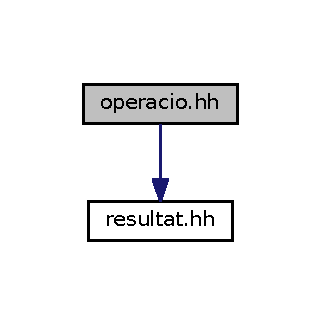
\includegraphics[width=154pt]{operacio_8hh__incl}
\end{center}
\end{figure}
\subsection*{Clases}
\begin{DoxyCompactItemize}
\item 
class \hyperlink{classoperacio}{operacio}
\begin{DoxyCompactList}\small\item\em Conté les operacions que s’han definit i les opera quan apareixen a una expressió \end{DoxyCompactList}\end{DoxyCompactItemize}

\hypertarget{resultat_8hh}{}\section{Referencia del Archivo resultat.\+hh}
\label{resultat_8hh}\index{resultat.\+hh@{resultat.\+hh}}
Dependencia gráfica adjunta para resultat.\+hh\+:\nopagebreak
\begin{figure}[H]
\begin{center}
\leavevmode
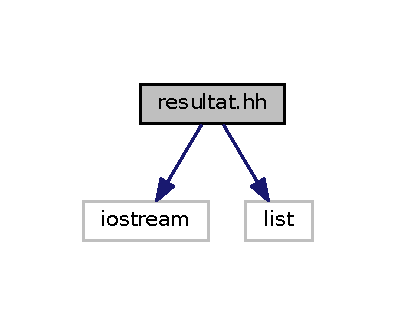
\includegraphics[width=190pt]{resultat_8hh__incl}
\end{center}
\end{figure}
\subsection*{Clases}
\begin{DoxyCompactItemize}
\item 
class \hyperlink{classresultat}{resultat}
\begin{DoxyCompactList}\small\item\em Objecte que representa el resultat d\textquotesingle{}una operació \end{DoxyCompactList}\end{DoxyCompactItemize}

\hypertarget{resultat__lectura_8hh}{}\section{Referencia del Archivo resultat\+\_\+lectura.\+hh}
\label{resultat__lectura_8hh}\index{resultat\+\_\+lectura.\+hh@{resultat\+\_\+lectura.\+hh}}
\subsection*{Clases}
\begin{DoxyCompactItemize}
\item 
class \hyperlink{classresultat__lectura}{resultat\+\_\+lectura}
\begin{DoxyCompactList}\small\item\em Guarda la informació necessària per entendre i tractar l’entrada de la pràctica. \end{DoxyCompactList}\end{DoxyCompactItemize}

\hypertarget{variable_8hh}{}\section{Referencia del Archivo variable.\+hh}
\label{variable_8hh}\index{variable.\+hh@{variable.\+hh}}
Dependencia gráfica adjunta para variable.\+hh\+:\nopagebreak
\begin{figure}[H]
\begin{center}
\leavevmode
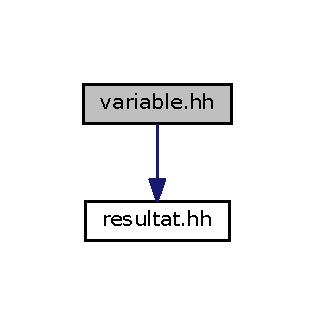
\includegraphics[width=287pt]{variable_8hh__incl}
\end{center}
\end{figure}
\subsection*{Clases}
\begin{DoxyCompactItemize}
\item 
class \hyperlink{classvariable}{variable}
\begin{DoxyCompactList}\small\item\em Conté les variables que s’han definit. \end{DoxyCompactList}\end{DoxyCompactItemize}

%--- End generated contents ---

% Index
\backmatter
\newpage
\phantomsection
\clearemptydoublepage
\addcontentsline{toc}{chapter}{Índice}
\printindex

\end{document}
